\section{Solar Coordinates - Will}
\label{sec:coords}
\cite{2006A&A...449..791T} defined a set of coordinate frames for use with solar physics data, and the transformations between them.  This work forms the basis of SunPy's solar physics coordinate systems.  The coordinates are implemented using \astropy's coordinate module, and extend \astropy's coordinate frame transform graph.  This makes it possible to easily transform between \sunpy solar physics-based coordinate frames and those implemented by \astropy.

Four solar physics coordinate frames are currently implemented, the \hpc, \hcc, \hgs, and \hgc coordinate systems.

Both \hpc and \hcc frames require that the location of the observer is defined. For example in Helioprojective the observer is at the origin of the coordinate system. This information is encoded in the Helioprojective and Heliocentric frames as the observer attribute, which is itself an instance of the HeliographicStonyhurst frame. The default observer location is set to the position of the Earth as long as the obstime attribute is specified. If the obstime attribute is not set then you will be unable to transform the frame unless an explicit observer is specified, as the time is required to calculate the location of the Earth. The location of the observer is automatically populated from meta data when coordinate frames are created using map.

Coordinates are great!

validation of coordinates with other sources (e.g. spice, solarsoft, stereo header?)

figure of solar coordinates graph (see astropy coordinates graph for example).

\begin{figure}
  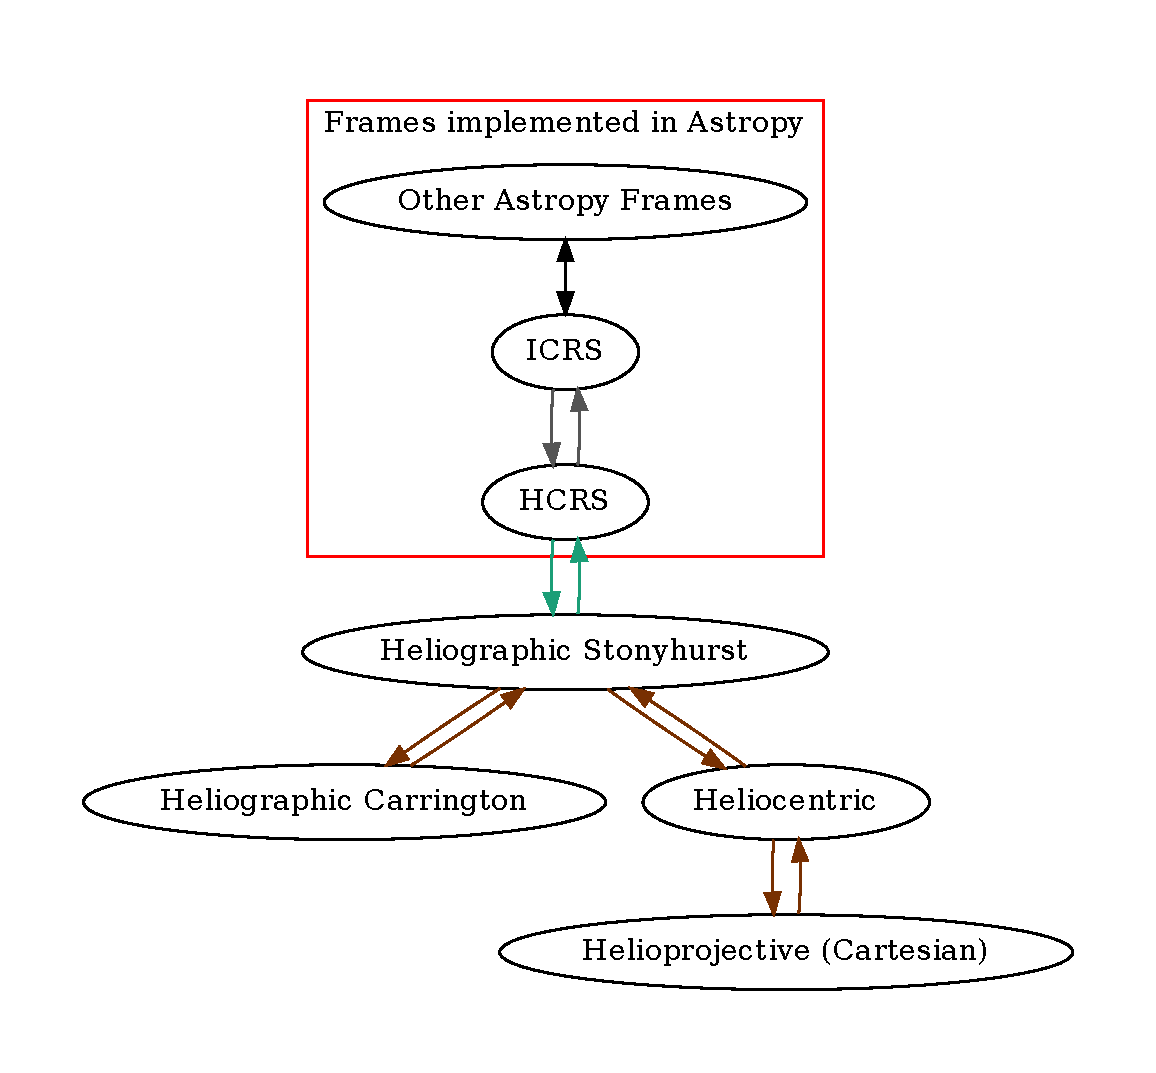
\includegraphics{figures/sunpy_frames.pdf}
\caption{TODO: Give this a legend for the transform types?}
\label{fig:image2}
\end{figure}

\begin{figure}
\center
  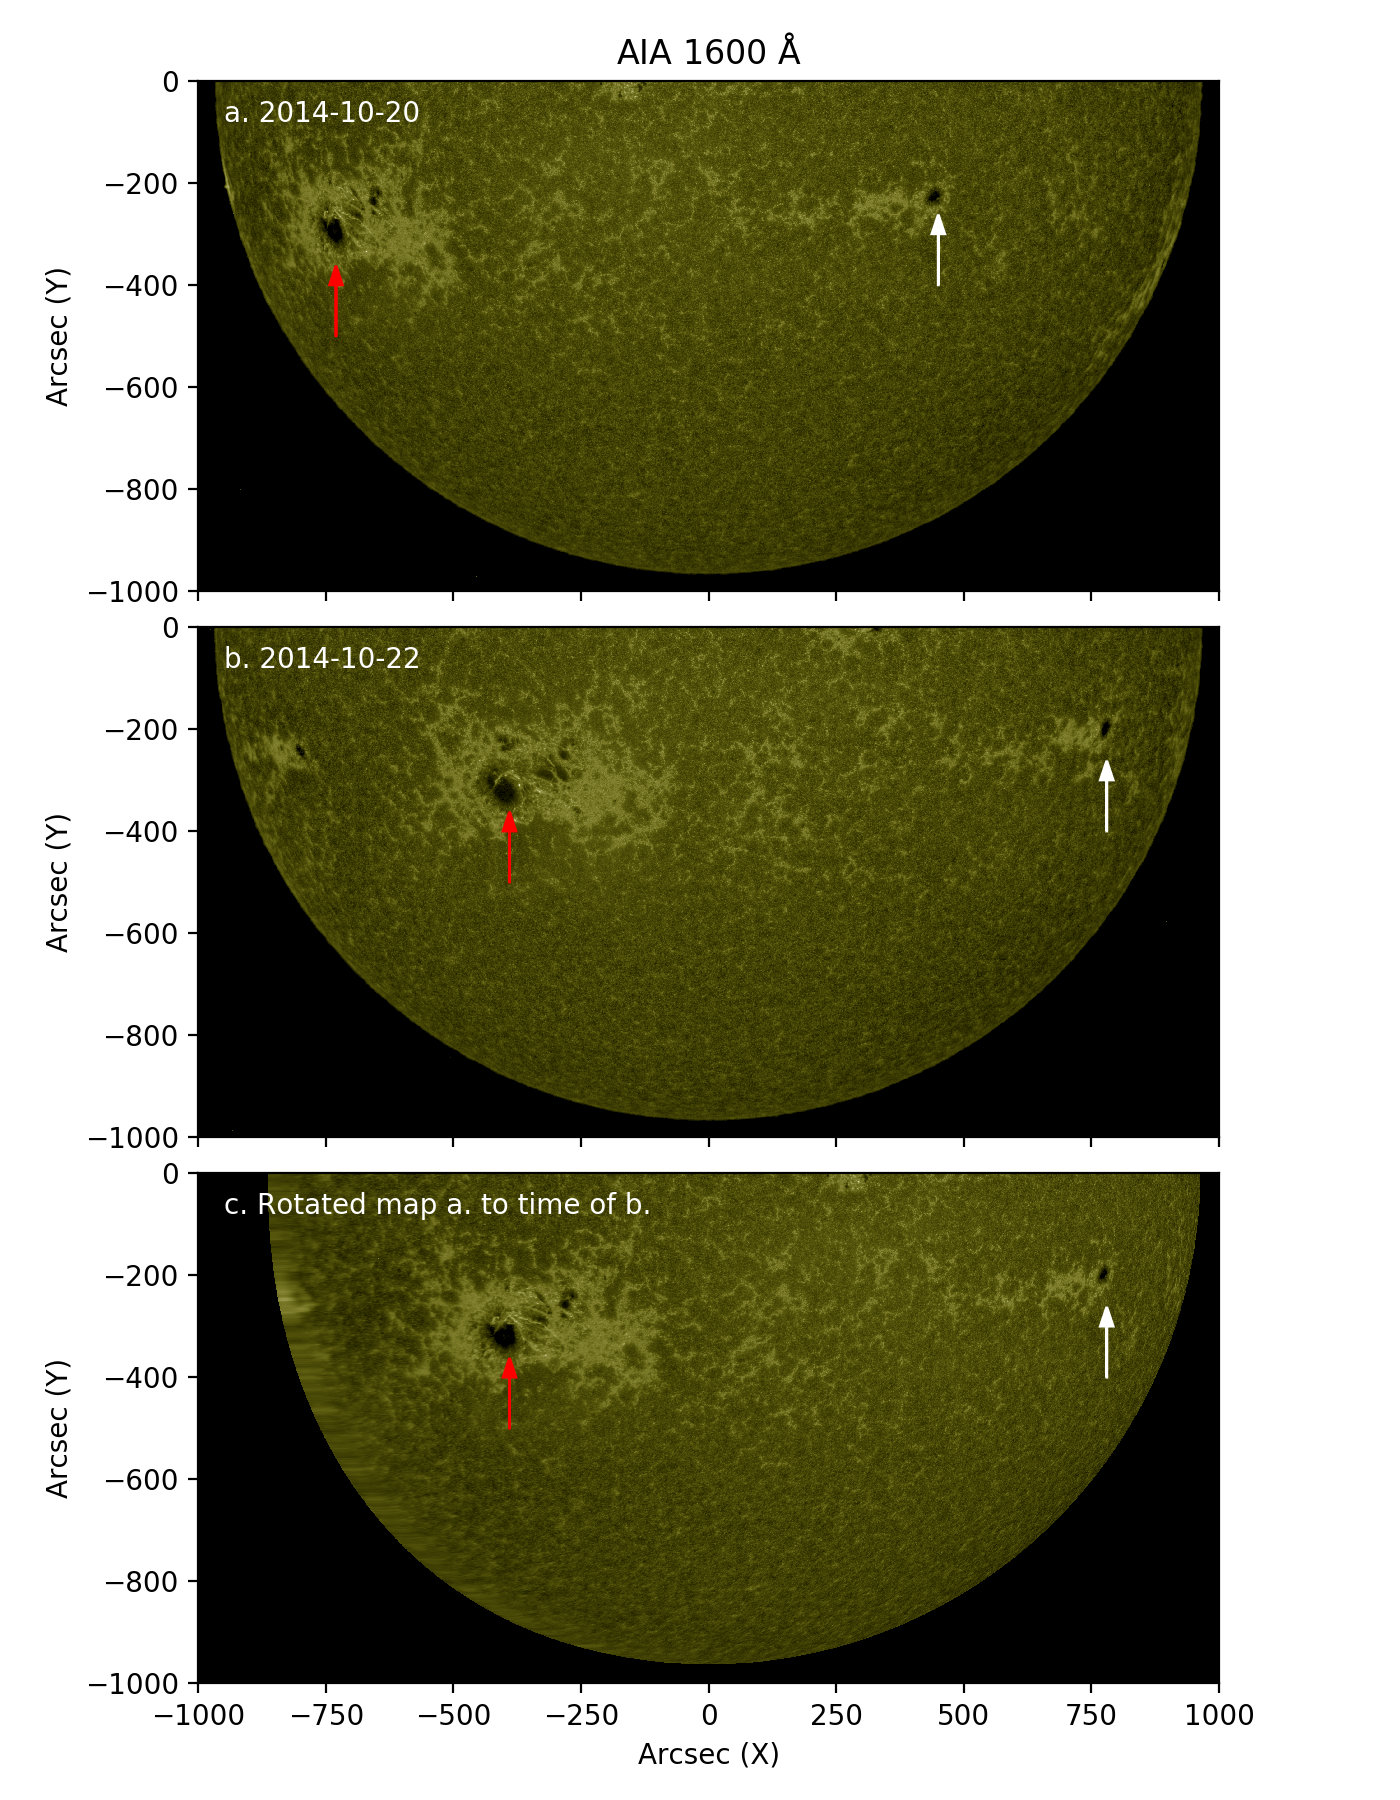
\includegraphics[width = 0.8\textwidth]{figures/diff_rot_aia1600.png}
\caption{Example of the functionality of \sunpy to apply solar differential rotation to a Map. Panels (a) and (b) show the Sun as observed in AIA 1600~\AA\ on two different days, 2014-02-20 and 2014-02-22. A large sunspot group is highlighted by the red arrow, and a smaller sunspot by the white arrow. Panel (c) shows the map of (a) that has been rotated differentially using \sunpy to the time of map (b).}
\label{fig:diff_rot}
\end{figure}